\chapter{Algorytmy sterowania}
\label{cha:ch7_algorytmy_sterowania}

Obsługa czujników odległości i bazowania, a także algorytmy sterowania, zostały zaimplementowane na przemysłowym sterowniku PLC Siemens S7-1211C. Schemat blokowy głównej pętli programu, uruchamianej co cykl procesora w bloku \texttt{OB1}, został przedstawiony na \cref{fig:schemat_petla_glowna_PLC}, natomiast szczegółowy opis poszczególnych elementów i algorytmów zamieszczono poniżej.

\begin{figure}[ht]
    \centering
    
    \begin{tikzpicture}[auto, node distance=1cm,>=latex']
    \node [roundblock] (start) {\textsc{START}};
    \node [block, below=of start] (sensors) {Odczyt czujników};
    \node [block, below=of sensors] (main_sequence) {Główna sekwencja};
    \node [block, below=of main_sequence] (outputs) {Zapis do wyjść};
    
    \draw [->] (start) -- (sensors);
    \draw [->] (sensors) -- (main_sequence);
    \draw [->] (main_sequence) -- (outputs);
    \draw [->] (outputs.west) -- ++ (-1,0) |- (sensors.west);
    \end{tikzpicture}
    
    \caption{Schemat pętli głównej programu.}
    \label{fig:schemat_petla_glowna_PLC}
\end{figure}

W ramach bloku \textit{Odczyt czujników} następują poniższe operacje:
\begin{itemize}
    \item obsługa enkodera:
    \begin{itemize}
        \item przeliczanie wartości licznika enkodera na kąt obrotu wału motoreduktora,
        \item przeliczanie kąta obrotu wału motoreduktora na kąt obrotu belki, zgodnie z informacjami podanymi w rozdziale \ref{sec:ch4_zaleznosc_kata_silnika_i_kata_belki},
    \end{itemize}
    \item obsługa czujników odległości:
    \begin{itemize}
        \item obliczanie odległości dla każdego czujnika przy wykorzystaniu punktów charakterystyki i~algorytmu aproksymacji liniowej,
        \item obliczanie pozycji kulki oraz jej średnicy,
        \item weryfikacja obecności kulki (szerzej opisana w rozdziale \ref{sec:ch7_wykrywanie_braku_kulki}),
    \end{itemize}
    \item generowanie impulsów od zboczy: narastającego dla przycisku \texttt{START} (NO) oraz opadającego dla przycisku \texttt{STOP} (NC),
    \item generowanie impulsu od opadającego zbocza czujnika bazowania.
\end{itemize}

W programie obsługiwane są tylko \num{3} wyjścia sterownika. Dwa z nich służą do sterowania silnikiem (sygnały \textit{PWM}, \textit{kierunek}), trzeci steruje diodą sygnalizacyjną. Sygnał \textit{PWM} kontrolowany jest przez sterownik jako tzw. wyjście pulsacyjne (\textit{PTO}); rolą programisty jest dostarczenie odpowiedniej wartości liczbowej do konkretnego słowa wyjściowego sterownika (tutaj \texttt{\%QW1000}). Częstotliwość wyjścia pulsacyjnego ustawiono na \SI{20}{\kilo\hertz}, natomiast kontrolę wypełnienia na setki, tzn. wpisanie wartości \num{85} do słowa wyjściowego sygnału PWM oznacza wypełnienie \SI{85}{\percent}.

Z racji możliwości sterowania obrotami silnika w dwie strony, regulator pozycji belki może zwrócić wartość z zakresu \numrange[range-phrase={ do }]{-100}{100}; stąd w bloku \textit{Zapis do wyjść} następuje konwersja tej wartości na jej moduł i zapis tego modułu do \texttt{\%QW1000}, natomiast sygnał \textit{kierunek} ustawiony jest na \num{1} dla ujemnej wartości sterowania, a na \num{0} dla dodatniej.

Równolegle do bloku \texttt{OB1}, wywoływanego co cykl procesora, użyto dwóch bloków organizacyjnych \texttt{OB30} i \texttt{OB31} wywoływanych co \SI{50}{\milli\second}. Rolą pierwszego z nich jest uruchamianie regulatorów (więcej w rozdziale \ref{sec:ch7_regulatory}), natomiast rolą drugiego jest obliczanie pochodnych sygnałów w czasie.

W \texttt{OB31} następuje obliczanie prędkości liniowej kulki oraz prędkości kątowej belki według następujących wzorów:
\begin{align*}
    v &= \frac{\Delta x}{\Delta t} \\
    \omega &= \frac{\Delta \alpha}{\Delta t}
\end{align*}
gdzie:
\begin{itemize}
    \item $\Delta t$ to stała wartość \SI{50}{\milli\second} równa okresowi wywołań bloku \texttt{OB31},
    \item $\Delta x$ to różnica wartości obecnej pozycji liniowej kulki oraz pozycji z poprzedniego wywołania bloku \texttt{OB31},
    \item $\Delta \alpha$ to różnica wartości obecnego kąta belki oraz kąta z poprzedniego wywołania bloku \texttt{OB31}.
\end{itemize}

%%%%
\section{Wykrywanie braku kulki}
\label{sec:ch7_wykrywanie_braku_kulki}

Jak to zostało wspomniane w rozdziale \ref{sec:ch5_identyfikacja_charakterystyk_czujnikow}, poza zebraniem charakterystyk czujników odległości dla kolejnych położeń kulki, sprawdzono również jak reagują czujniki, gdy pomiędzy nimi nie znajduje się żadna przeszkoda.

Pomiary przedstawiono na \cref{fig:czujniki_charakterystyka_bez_przeszkody}. Wynika z nich, że oba czujniki przy braku przeszkody mocno szumią; jednocześnie widać, że średnie sygnałów to około \num{700} i niecałe \num{500}, a także widać sporadyczne skoki (zwłaszcza czujnika lewego) do wartości w zakresie charakterystyk (por. \cref{fig:aproksymacja_czujnika_lewego}).

Biorąc powyższe fakty pod uwagę, zdecydowano się na następujący algorytm wykrywania obecności kulki pomiędzy czujnikami:
\begin{itemize}
    \item jeżeli wartość z przetwornika ADC czujnika lewego wynosi mniej niż \num{800} oraz wartość z przetwornika ADC czujnika prawego wynosi mniej niż \num{600}, to zresetuj zmienną binarną \textit{kulka obecna},
    \item jeżeli wartość z przetwornika ADC czujnika lewego wynosi więcej niż \num{900} oraz wartość z przetwornika ADC czujnika prawego wynosi więcej niż \num{900}, to ustaw zmienną binarną \textit{kulka obecna}.
\end{itemize}

W wyniku zastosowania powyższych warunków, błędnie określona obecność kulki będzie tylko w~sytuacji chwilowego wystąpienia skoków wartości na obu czujnikach; brak kulki zostanie wykryty natychmiast po zaniknięciu obu skoków wartości.

\begin{figure}[ht]
    \centering
    \includesvg[width=1\textwidth,svgpath=./vector_graphics/]{bez_przeszkody}    
    \caption{Odpowiedź czujników odległości, gdy pomiędzy nimi nie ma żadnej przeszkody.}
    \label{fig:czujniki_charakterystyka_bez_przeszkody}
\end{figure}

%%%%
\section{Sekwencja główna programu}
\label{sec:sekwencja_glowna}

Sterownik PLC Siemens z serii S7-1200 nie obsługuje języka sterowania sekwencyjnego \textsc{S7-GRAPH}, który został zastrzeżony przez producenta tylko dla mocniejszej serii S7-1500 (\cite{SCL_S71200_S71500}). W~związku z~tym w~języku obsługiwanym przez S7-1200 (diagram drabinkowy \textit{LAD} \cite{PROGRAMOWANIE_PLC}) zaimplementowano okrojoną wersję sterowania sekwencyjnego, przedstawioną na \cref{fig:schemat_sekwencji}.

\begin{figure}[ht]
    \centering
    
    \begin{tikzpicture}[auto, node distance=1cm,>=latex']
    \node [startblock] (S1) {Bazowanie};
    \node [block, below=1.25of S1] (S2) {Oczekiwanie na przycisk};
    \node [block, below=2of S2] (S3) {Stabilizacja kulki w położeniu zerowym};
    \node [block, below=1.25of S3] (S4) {Identyfikacja systemu belki};
    \node [block, below=2of S4] (S5) {Identyfikacja systemu kulki};
    \node [block, below=2of S5] (S6) {Zmiana regulatorów na zidentyfikowane};
    
    \draw [->] (S1) -- node [] {$T_1$} (S2);
    \draw [->] (S2) -- node [pos=0.25,name=T2_1] {} node [pos=0.70] {$\uparrow$\texttt{START}} (S3);
    \draw [->] (T2_1.west) -| ++ (-2.5,1.5) node [left] {$\downarrow$\texttt{STOP}} |- (S1.west);
    \draw [->] (S3) -- node [] {$\uparrow$\texttt{START}, brak kulki} (S4);
    \draw [->] (S4) -- node [pos=0.25,name=T4_3] {} node [pos=0.70] {$T_4$} (S5);
    \draw [->] (S5) -- node [pos=0.25,name=T5_3] {} node [pos=0.70] {$T_5$} (S6);
    \draw [->] (T4_3.west) -| ++ (-3.5,1.5) node [left] {$\downarrow$\texttt{STOP}} |- (S3.185);
    \draw [->] (T5_3.west) -| ++ (-5,2) node [left] {$\downarrow$\texttt{STOP}} |- (S3.175);
    \draw [->] (S6.east) -| ++ (1.5,4) node [right] {$T_6$} |- (S3);
    \end{tikzpicture}
    
    \caption{Schemat sterowania sekwencyjnego zaimplementowanego w sterowniku PLC.}
    \label{fig:schemat_sekwencji}
\end{figure}

Na schemacie sekwencji z \cref{fig:schemat_sekwencji} wyróżnić można:
\begin{itemize}
    \item stany, oznaczone jako prostokąty, w tym stan początkowy (prostokąt z podwójnym obramowaniem),
    \item tranzycje, widoczne jako połączenia między stanami przy użyciu strzałek,
    \item warunki tranzycji umieszczone obok strzałek, oznaczone przy użyciu symbolu $T_i$ lub przy użyciu faktycznie wykorzystanych warunków logicznych.
\end{itemize}

Względem symboliki powszechnie stosowanej w językach sterowania sekwencyjnego (\cite{SEKW1}\cite{SEKW2}), na \cref{fig:schemat_sekwencji} brakuje działań. Zostało to zrobione umyślnie, gdyż każde działanie wiąże się z dłuższym algorytmem lub, jak w przypadku bazowania, równoległym grafem sekwencji, a zatem wpisanie ich obok bloków stanów wpłynęłoby negatywnie na czytelność schematu.

% TODO: uaktualnij wyrażenie w przy T_6
Na schemacie sekwencji na \cref{fig:schemat_sekwencji} wyróżnione zostały następujące warunki tranzycji:
\begin{itemize}
    \item $\downarrow$\texttt{STOP} oznacza zbocze opadające na sygnale z przycisku \texttt{STOP},
    \item analogicznie $\uparrow$\texttt{START} oznacza zbocze narastające na sygnale z przycisku \texttt{START},
    \item $T_1$ -- stan wysoki na rejestrze binarnym \texttt{M\_homed} oznaczającym wybazowanie wału motoreduktora,
    \item $T_4$ -- pomyślne zakończenie procesu identyfikacji belki,
    \item $T_5$ -- pomyślne zakończenie procesu identyfikacji kulki,
    \item $T_6$ -- uaktualnienie (zmiana) regulatorów używanych w systemie lub ich nastaw.
\end{itemize}

% TODO: zaktualizuj referencję
Poszczególne stany wymienione na \cref{fig:schemat_sekwencji} i uruchamiane w nich działania opisane zostały poniżej (proces bazowania, regulator pozycji belki i regulator stabilizujący kulkę w położeniu zerowym) oraz w rozdziale \ref{cha:ch8_algorytmy_samostrojenia} (identyfikacja systemu kulki, belki oraz przeprowadzone na ich podstawie samostrojenie).

%%%%
\section{Bazowanie}
\label{sec:ch7_bazowanie}

W wyniku zastosowania w obiekcie enkodera inkrementalnego bez pamięci, za każdym razem po uruchomieniu sterownika PLC konieczne jest przeprowadzenie procedury bazowania w~celu wykrycia położenia kątowego wału motoreduktora. Schemat procedury bazowania został przedstawiony na \cref{fig:schemat_bazowania}.

% TODO: znajdź źródło!!!
W procesie bazowania istotne jest najechanie na czujnik krańcowy (bazowania) zawsze od tej samej strony. Ta konieczność spowodowana jest obecnością luzów na przekładniach i dotyczy większości układów mechanicznych, w których użyto przekładni.

Dzięki zastosowaniu mechanizmu obrotowego, algorytm bazowania jest uproszczony, tzn. możliwe było zrezygnowanie z cofania się (obrotu w przeciwnym kierunku) wału w sytuacji, gdy znajduje się on na pozycji zasłaniającej czujnik bazowania. Zamiast tego wystarczy reakcja na zbocze opadające sygnału z czujnika.

\begin{figure}[ht]
    \centering
    
    \begin{tikzpicture}[auto, node distance=1cm,>=latex']
    \node [roundblock] (S1) {Start};
    \node [conditionblock, below=1of S1] (S2) {Czy enkoder jest wybazowany?};
    \node [block, below=1of S2] (S3) {Ustaw niską wartość napięcia sterującego silnikiem};
    \node [conditionblock, below=1of S3] (S4) {Czy nastąpiło zbocze opadające na czujniku bazowania?};
    \node [block, below=1of S4] (S5) {Ustaw zerowe napięcie sterujące silnikiem};
    \node [block, below=1of S5] (S6) {Ustaw bit wybazowania enkodera};
    \node [block, below=1of S6] (S7) {Ustaw wartość licznika enkodera};
    \node [roundblock, below=1of S7] (S8) {Stop};
    
    \draw [->] (S1) -- (S2);
    \draw [->] (S2.west) -| ++ (-2,0) node [above right] {Tak} |- (S8);
    \draw [->] (S2) -- node [] {Nie} (S3);
    \draw [->] (S3) -- (S4);
    \draw [->] (S4) -- node [] {Tak} (S5);
    \draw [->] (S4.east) -| ++ (2,0) node [above left] {Nie} |- (S3);
    \draw [->] (S5) -- (S6);
    \draw [->] (S6) -- (S7);
    \draw [->] (S7) -- (S8);
    \end{tikzpicture}
    
    \caption{Schemat blokowy algorytmu bazowania licznika enkodera.}
    \label{fig:schemat_bazowania}
\end{figure}

W momencie wystąpienia zbocza opadającego sygnału z czujnika bazowania następuje ustawienie wartości \num{149} w liczniku enkodera oraz ustawienie stanu wysokiego w rejestrze \textsc{M\_homed}, używanym m.in. przez sekwencję główną.

%%%%
\section{Regulatory}
\label{sec:ch7_regulatory}

Jak to zostało wspomniane we wstępie do rozdziału, obliczanie nowych wartości sterowania z obu regulatorów umieszczone zostało w bloku \texttt{OB30} wywoływanym przez sterownik PLC z okresem \SI{50}{\milli\second}.

Wywoływanie regulatorów z określoną częstotliwością ma swoje podłoże w regulacji typu PID. Oprogramowanie \textsc{Siemens TIA Portal}, jak również sterowniki serii S7-1200, obsługuje tak zwane obiekty technologiczne (\cite{S7MANUAL}\cite{SCL_S71200_S71500}); jednym z nich jest prosty regulator typu PID z mechanizmem automatycznego strojenia. Blok takiego obiektu technologicznego musi być wywoływany w programie sterownika z określoną częstotliwością, co związane jest z koniecznością liczenia pochodnych sygnału uchybu w czasie.

Umieszczenie regulatorów w bloku \texttt{OB30} umożliwia zatem przeprowadzenie łatwej zamiany na obiekt technologiczny PID gdyby nastała taka konieczność.

Ponadto sygnały, z których korzystają regulatory, takie jak prędkość obrotowa belki czy prędkość liniowa kulki, również są liczone z~okresem \SI{50}{\milli\second}, co oznacza, że nie należy uruchamiać bloku \texttt{OB30} ani rzadziej (co powodowałoby pracę ze zbyt starymi wartościami sygnałów), ani częściej (co powodowałoby duże opóźnienie w reakcji regulatora).

Regulatory opisane w rozdziałach \ref{sec:ch6_regulator_belki} oraz \ref{sec:ch6_regulator_kulki} są regulatorami typu proporcjonalnego od stanu, co oznacza, że ich implementacja w sterowniku PLC jest równoznaczna z obliczeniem sumy sygnałów od stanu wymnożonych przez macierz współczynników. W przypadku obu regulatorów, uzyskano to za pomocą bloku \texttt{Calculate} (\cref{fig:tia_portal_blok_calculate}), umożliwiającego zdefiniowanie prostych wyrażeń algebraicznych.

\begin{figure}[h]
    \centering
    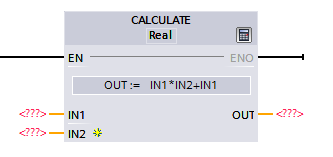
\includegraphics[width=0.5\textwidth]{tia_calculate_block}
    \caption{Zrzut ekranu z programu \textsc{Siemens TIA Portal} z widocznym blokiem \texttt{Calculate} i przykładowym równaniem, które ten blok może obliczyć.}
    \label{fig:tia_portal_blok_calculate}
\end{figure}

% TODO: eksperyment regulacji poprzez obiekt technologiczny PID -- może próba przeprowadzenia samostrojenia?

%%%%
\subsection{Regulator położenia belki}
\label{subsec:ch7_regulator_belki}

Regulator podrzędny, odpowiedzialny za ustawienie belki w zadanym miejscu, realizuje obliczanie napięcia podanego na silnik według wzoru \eqref{eq:regulator_belki_wzor}:
\begin{equation}
    u = K_b(1) \cdot \epsilon_\alpha + K_b(2) \cdot \epsilon_\omega
    \label{eq:regulator_belki_wzor}
\end{equation}
gdzie $K_b$ to macierz wzmocnień regulatora (opisana w rozdziale \ref{sec:ch6_regulator_belki}), a $\epsilon_\alpha$ i $\epsilon_\omega$ to odpowiednio odchyłka położenia kątowego belki i jej prędkości kątowej od zadanych przez regulator nadrzędny wartości.

Należy zwrócić uwagę, że realizacja powyższego wzoru na sterowniku PLC wymaga przeskalowania napięcia $u$ na wypełnienie sygnału PWM. W tym celu zastosowano skalowanie liniowe o współczynniku kierunkowym $\frac{100}{11,95}=8,3682$, gdzie \num{100} to maksymalna wartość wypełnienia PWM, a \num{11,95} to napięcie znamionowe, które zostało użyte w modelu symulacyjnym silnika (rozdział \ref{sec:ch4_model_silnika}).

%%%%
\subsection{Regulator położenia kulki}
\label{subsec:ch7_regulator_kulki}

Regulator nadrzędny, nazywany regulatorem położenia kulki, ma za zadanie generować sterowanie dla regulatora podrzędnego według wzoru \eqref{eq:regulator_kulki_wzor}:

\begin{nalign}
    \alpha_\text{ref} &= K_k(1) \cdot \epsilon_1 + K_k(2) \cdot \epsilon_2 + K_k(3) \cdot \epsilon_3 + K_k(4) \cdot \epsilon_4 \\
    \omega_\text{ref} &= K_k(5) \cdot \epsilon_1 + K_k(6) \cdot \epsilon_2 + K_k(7) \cdot \epsilon_3 + K_k(8) \cdot \epsilon_4
    \label{eq:regulator_kulki_wzor}
\end{nalign}
gdzie $K_k$ to macierz wzmocnień regulatora (opisana w rozdziale \ref{sec:ch6_regulator_kulki}), $\alpha_\text{ref}$ oraz $\omega_\text{ref}$ są wartościami zadanymi dla regulatora podrzędnego, a $\epsilon_i, ~i=1\dots4$ to odchyłki wartości stanów systemu od ich wartości zadanych.

% bez sensu te limity bo nic nie dają realistycznego
%% TODO: zmierzyć prędkość kątową?
%Wartości wyjściowe z tego regulatora $\alpha_\text{ref}$ oraz $\omega_\text{ref}$ zostały przeskalowane za pomocą pary bloków \texttt{Limit} tak, że nie wykraczają poza fizyczne możliwości ruchu belki (\SI{+-0,3}{\radian} dla pozycji kątowej i \SI{+-58}{\radian\per\second} dla prędkości kątowej).

%%%%
\section{Podsumowanie}

W niniejszym rozdziale przedstawiono sposób obsługi oprzyrządowania obiektu regulacji (w tym czujników odległości i bazowania, przycisków oraz diody), a także szczegóły implementacyjne sterowania silnikiem przez mostek H i sygnały generowane na wyjściach sterownika PLC. Następnie opisano zadania bloków organizacyjnych \texttt{OB1}, \texttt{OB30} i \texttt{OB31} sterownika w obliczaniu pochodnych sygnałów, wyjścia z regulatorów czy pętli głównej programu.

W dalszej części rozdziału przedstawiono wykorzystane algorytmy wykrywania braku kulki, bazowania czy implementację regulatorów. Opisano również schemat sekwencji głównej programu.

%---------------------------------------------------------------------------